\chapter{Experimentos}
\label{cap:capitulo6}

\begin{flushright}
\begin{minipage}[]{10cm}
\emph{El verdadero método de conocimiento es el experimento.}\\
\end{minipage}\\

William Blake\\
\end{flushright}

\vspace{1cm}

En este capítulo se tratarán los diferentes experimentos que se han realizado para depurar las distintas funcionalidades del sistema, gracias a los cuales ha sido posible alcanzar los objetivos definidos en la Sección~\ref{sec:Requisitos}.


\section{Impresión 3D}
\label{sec:Impresión 3D}

Uno de los primeros pasos para la construcción física del robot consistió en el diseño e impresión de las piezas estructurales. En el diseño se intentó minimizar el número de piezas con el objetivo de simplificar el montaje y reducir posible problemas de ensamblaje.


Sin embargo, durante la preparación de las piezas para su impresión se detectó un problema debido a las limitaciones  del tamaño máximo de fabricación de la impresora utilizada. Como se puede observar en la Figura \ref{fig:impresion_vis}, algunas piezas superaban las dimensiones máximas permitidas por el área de impresión disponible.

\vspace{0.2cm}

\begin{figure}[H]
  \begin{center}
    \subcapcentertrue
    \subfigure[Pieza hacia arriba]{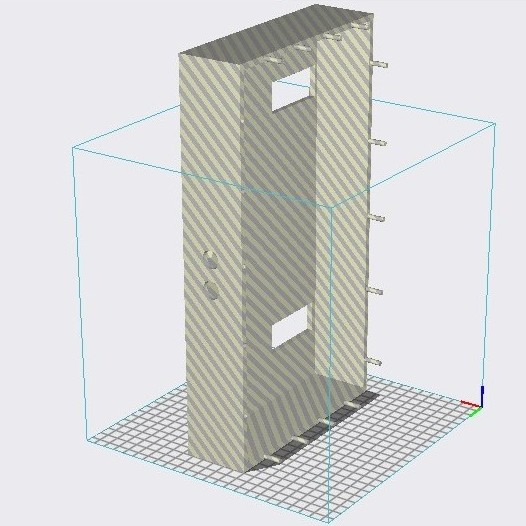
\includegraphics[width=0.48\textwidth, height=50mm, keepaspectratio=false]{figs/impresion}}
    \hspace{3mm}
    \subfigure[Pieza hacia abajo]{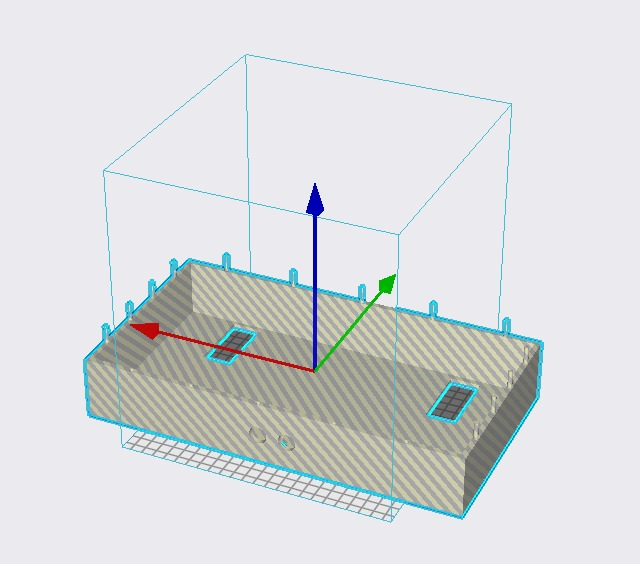
\includegraphics[width=0.48\textwidth, height=50mm, keepaspectratio=false]{figs/impresion2}}
  \end{center}
  \caption{Piezas 3D}
  \label{fig:impresion_vis}
\end{figure}

Para solventar este contratiempo se modificó el diseño original, dividiendo las piezas de mayor tamaño en varias piezas.

\vspace{0.2cm}

Una vez realizados los cambios, se inició la impresión de las distintas piezas  que componen la estructura del robot (Figura \ref{fig:piezas}).

\vspace{0.2cm}


\begin{figure} [h!]
  \begin{center}
    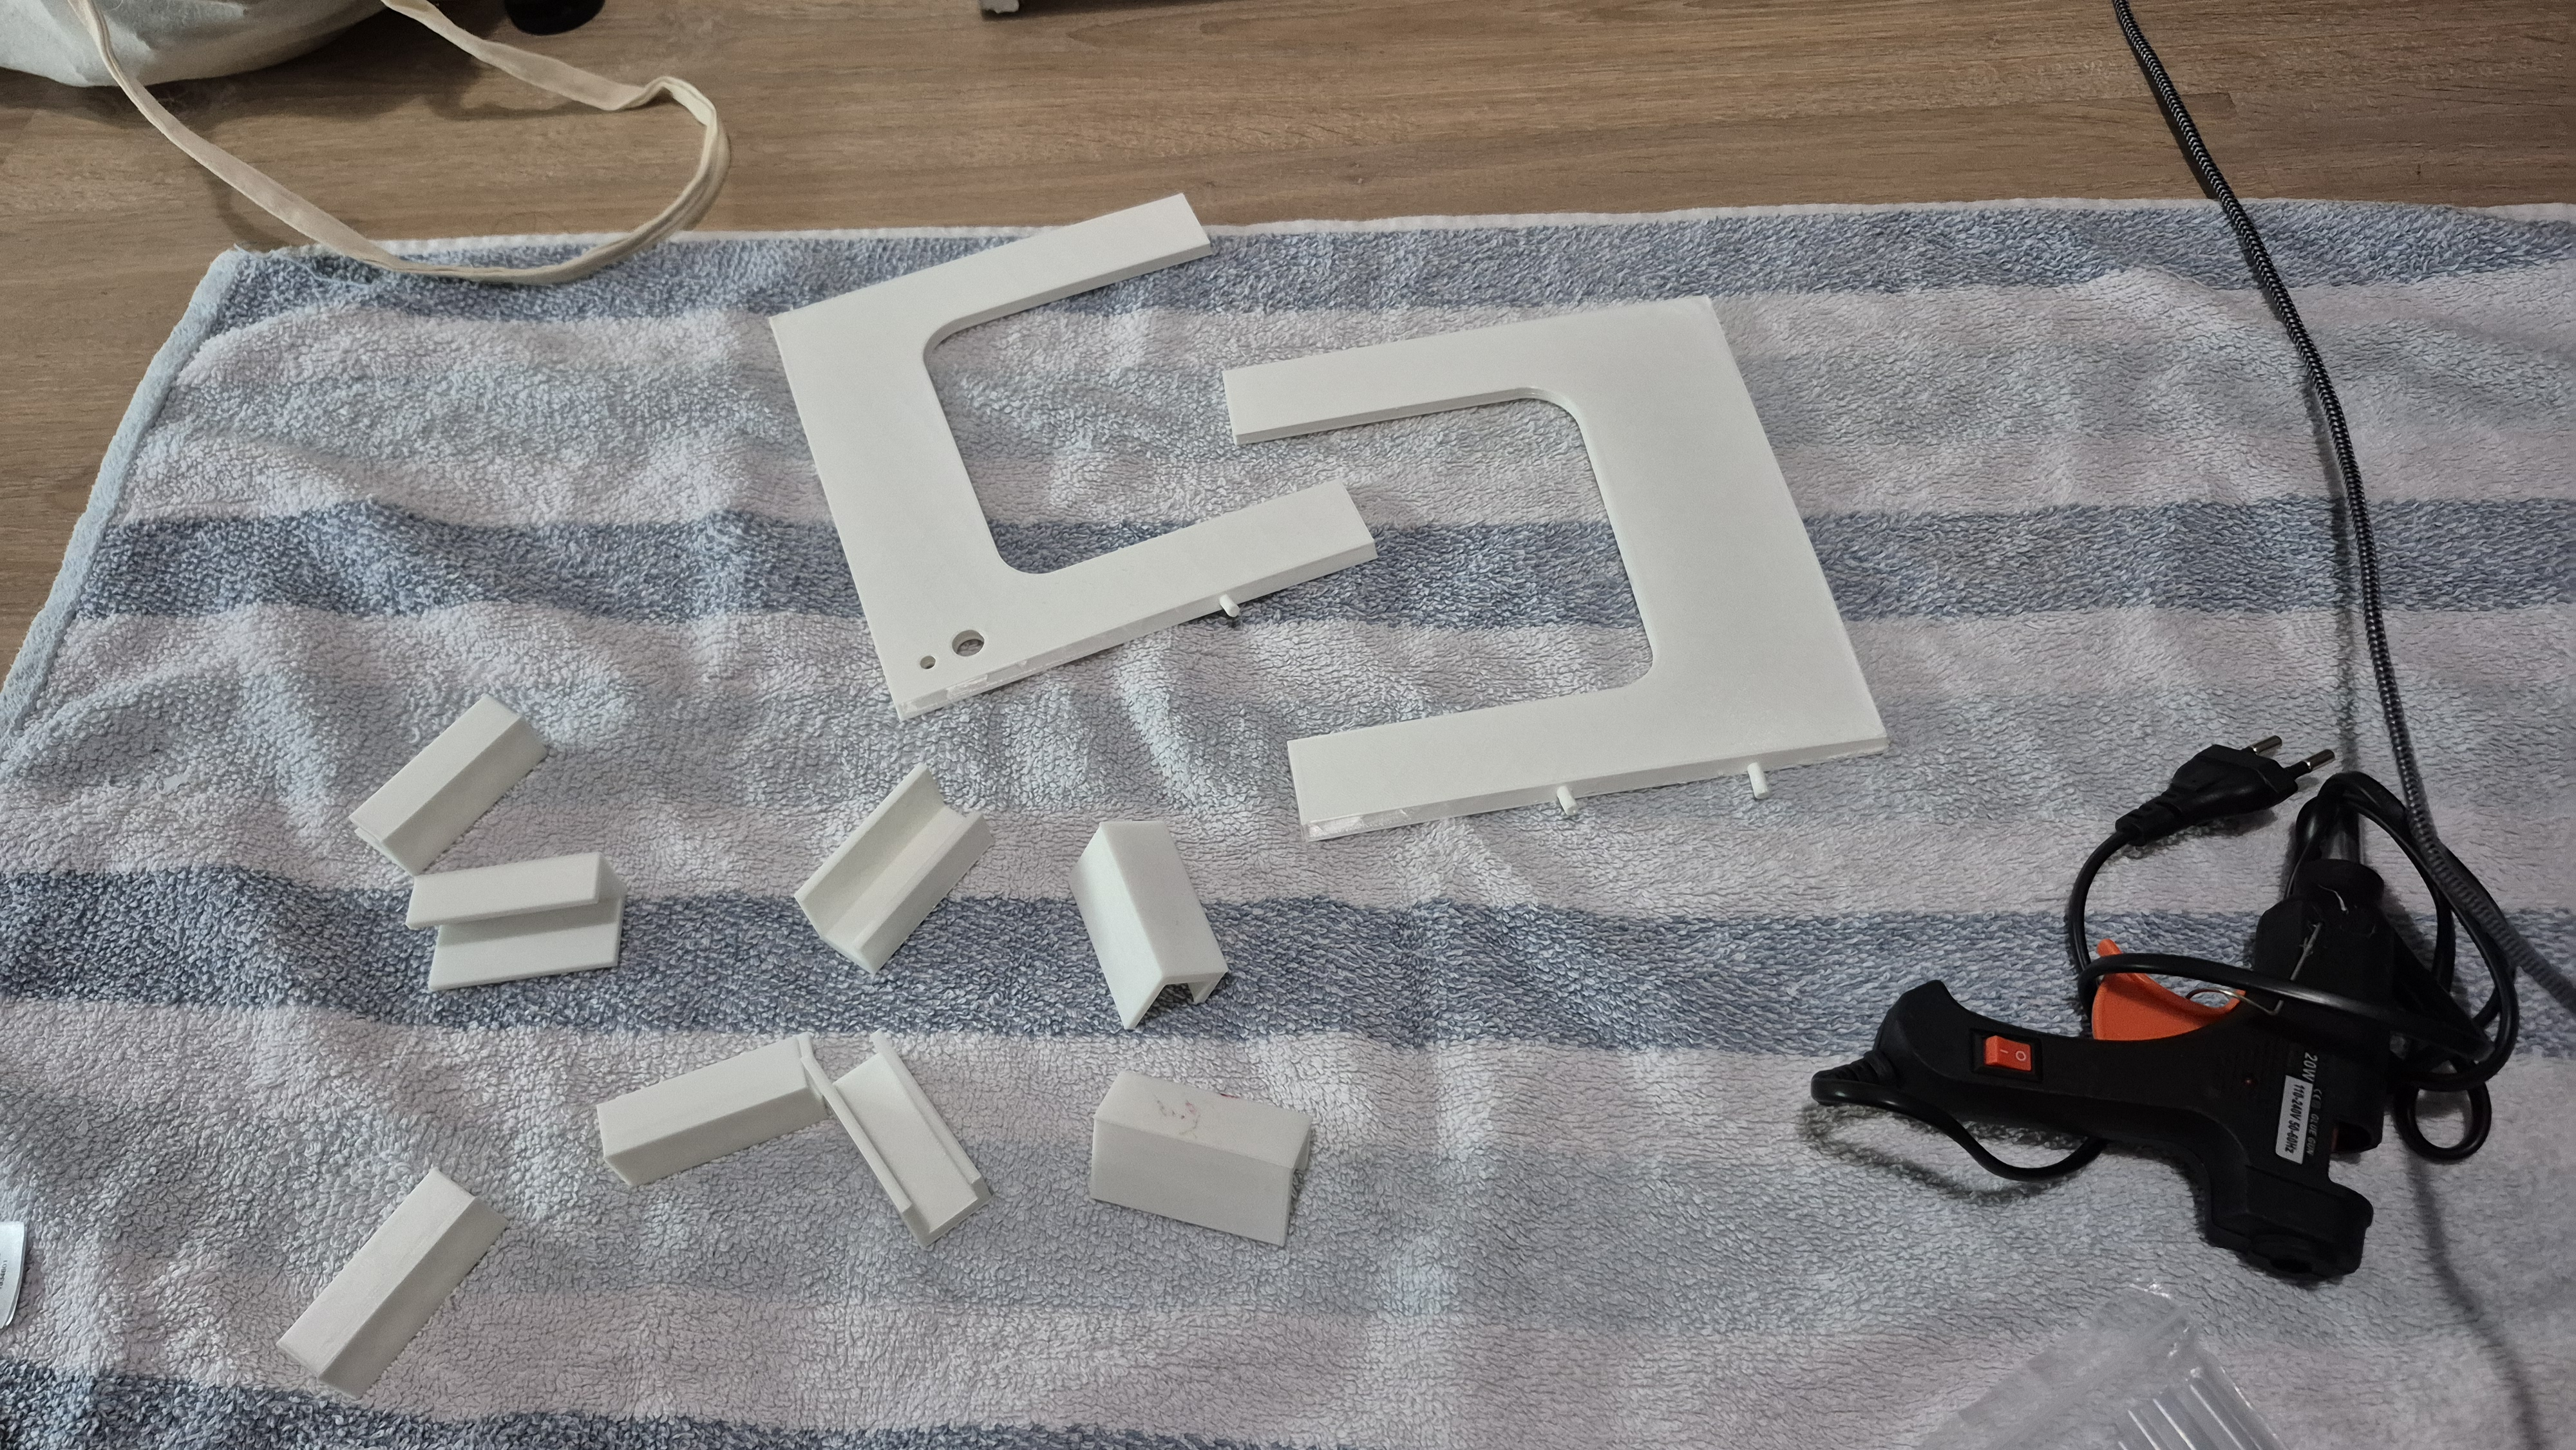
\includegraphics[width=12cm]{figs/piezas}
  \end{center}
  \caption{Piezas 3D impresas}
  \label{fig:piezas}
\end{figure}\


Tras la impresión de las piezas, y durante el montaje del robot, se detectaron dos problemas importantes. Por una parte, algunas dimensiones habían sido calculadas de forma incorrecta, por lo que no se disponía del espacio suficiente para integrar determinados componentes \textit{hardware} en el interior de la estructura.

Por este motivo fue necesario realizar modificaciones sobre algunas piezas impresas, ampliando huecos mediante procesos de lijado y aplicación de color. La Figura \ref{fig:sol} muestra una de las piezas modificadas durante esta fase.

\vspace{0.2cm}


\begin{figure} [h!]
  \begin{center}
    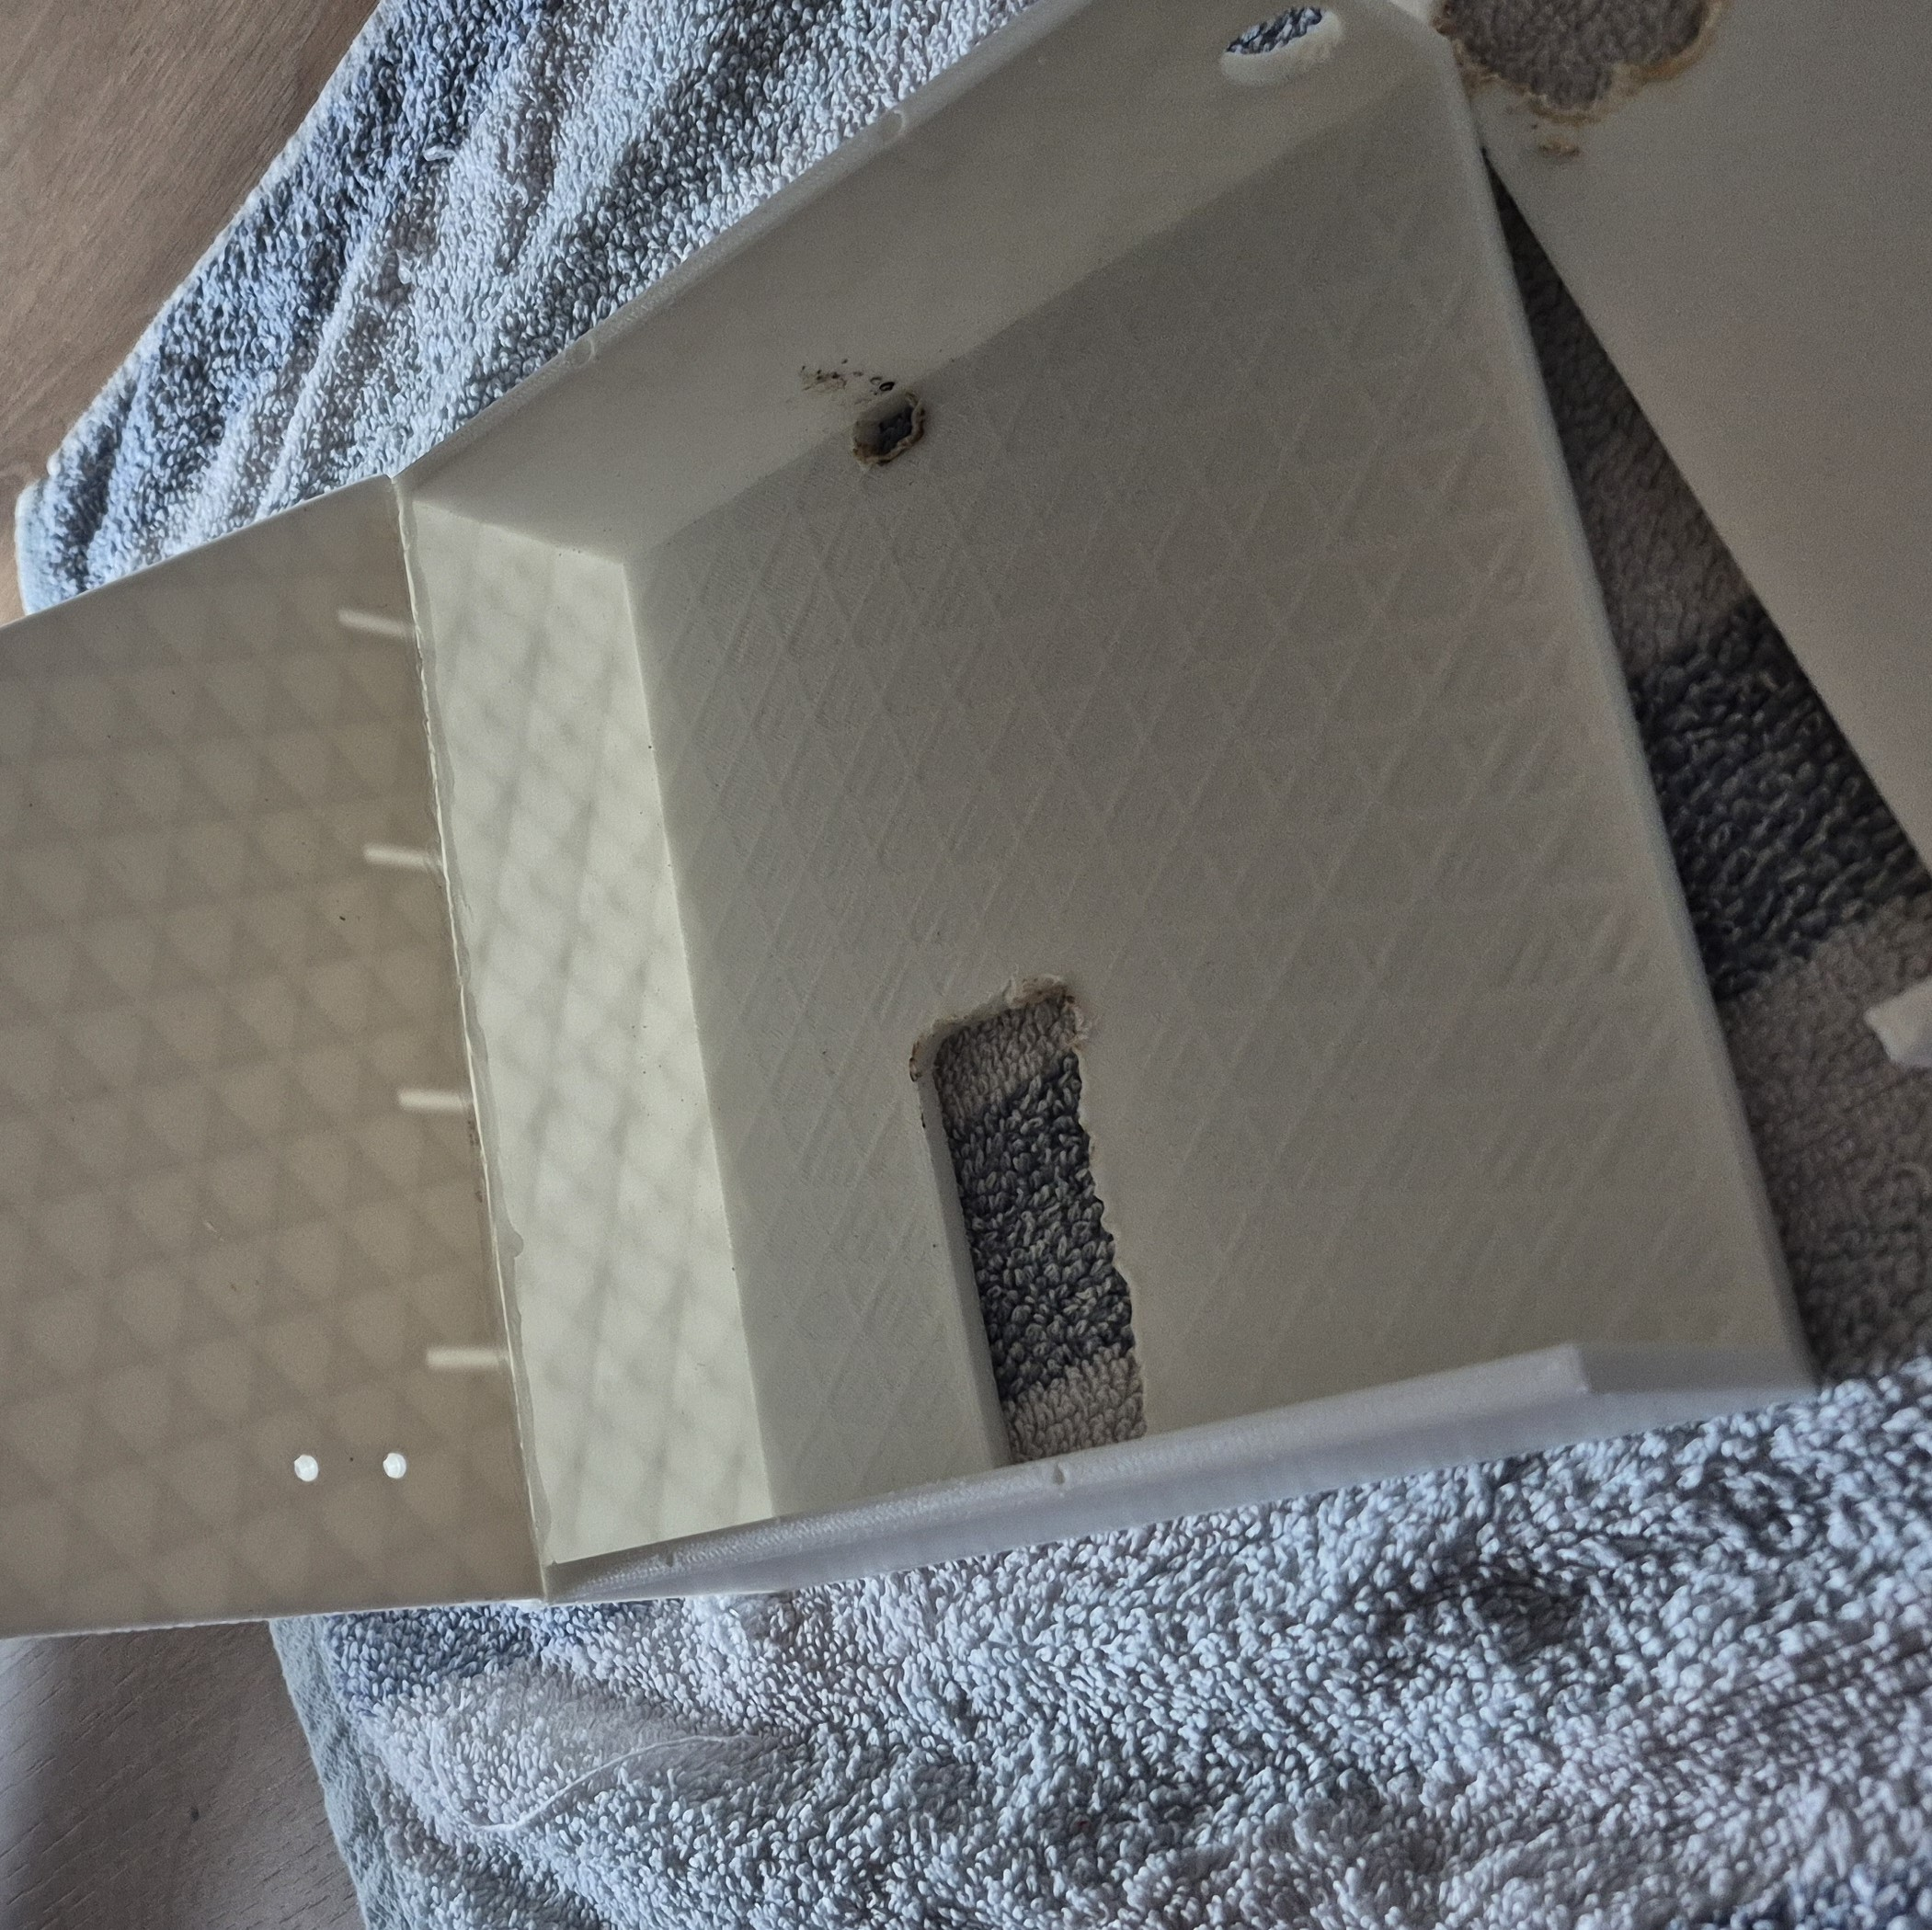
\includegraphics[width=8cm]{figs/sol}
  \end{center}
  \caption{Pieza modificada}
  \label{fig:sol}
\end{figure}\

Por otra parte, el diseño CAD incorporaba una serie de salientes destinados a encajar en los huecos de las piezas adyacentes, facilitando así el montaje de la estructura. Sin embargo, durante la impresión se observó que dichos salientes presentaban una superficie de contacto insuficiente con la pieza principal. Como consecuencia, varios de ellos se desprendieron durante la impresión.

Debido a este inconveniente, se descartó el sistema de encaje inicial y se optó por una solución alternativa basada en la utilización de adhesivo termofusible para el ensamblaje de las distintas piezas.


Se realizaron entonces una serie de modificaciones sobre el diseño original con el objetivo de adaptar la estructura a los inconvenientes encontrados durante el proceso de impresión y ensamblaje. Estas modificaciones permitieron integrar correctamente los componentes \textit{hardware} y obtener una estructura funcional del robot. En la Figura \ref{fig:estructura1} se muestra el resultado final de la estructura.

\vspace{0.2cm}

\begin{figure} [h!]
  \begin{center}
    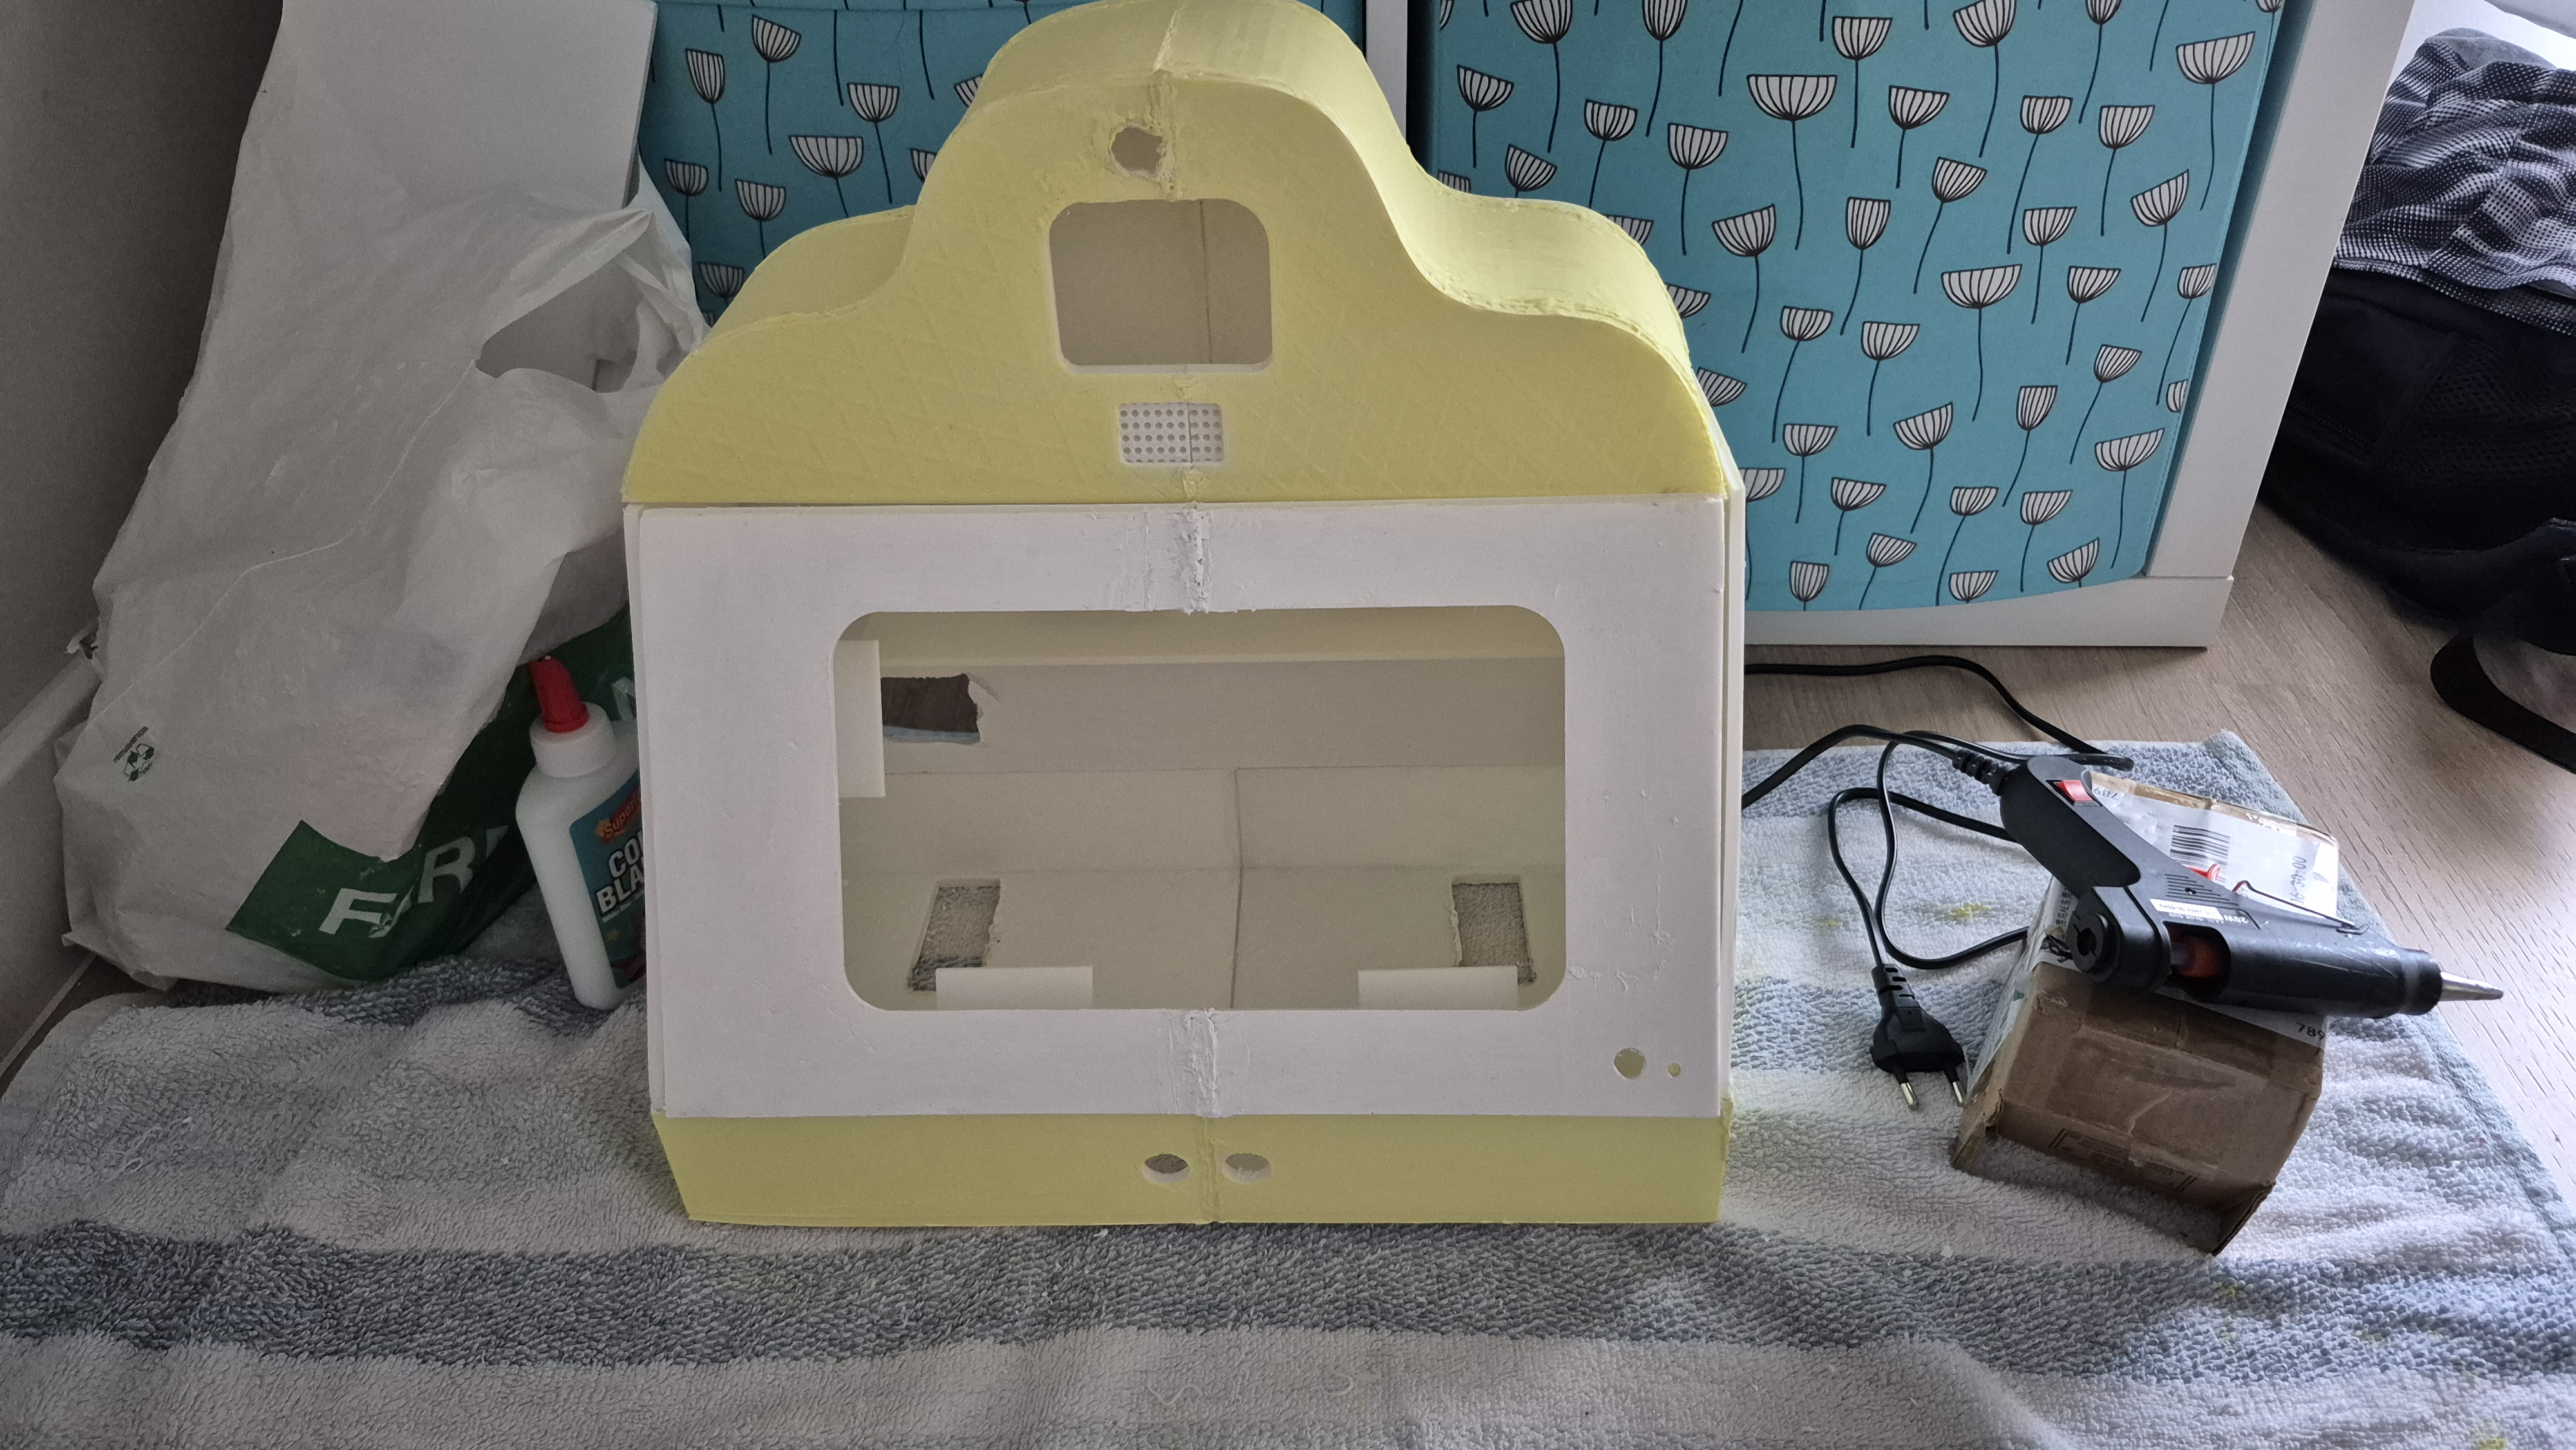
\includegraphics[width=12cm]{figs/estructura}
  \end{center}
  \caption{Estructura final del robot}
  \label{fig:estructura1}
\end{figure}\



\section{Alimentación del sistema}
\label{sec:Alimentación del sistema}

Durante la integración \textit{hardware} se observó que la Raspberry Pi era incapaz de alimentar correctamente todos los componentes electrónicos conectados al sistema. La incorporación de periféricos como la cámara o la pantalla táctil provocaban una elevada demanda energética, afectando al funcionamiento del robot.

\vspace{0.2cm}

Con el objetivo de identificar el origen del problema, se empleó un multímetro para comprobar la tensión suministrada por la fuente de alimentación utilizada inicialmente, obteniéndose un valor 4.9 V, inferior a los 5V recomendados para el correctamente funcionamiento de la Raspberry Pi. Así que hubo que sustituir el cargador original por una nueva fuente de alimentación capaz que proporcionar una tensión estable de 5V.

No obstante, el reemplazo de la fuente de alimentación no fue suficiente para resolver completamente el problema. Dado que la mayoría de componentes continuaban conectados a la Raspberry Pi, esta no era capaz de funcionar correctamente debido a la elevada carga energética que soportaba. Como solución, se incorporó un HUB USB con alimentación externa, al que se conectaron algunos periféricos del robot. De este modo, dichos dispositivos reciben la energía directamente del HUB, mientras que la Raspberry solo se encarga del intercambio de datos.

\vspace{0.2cm}

Gracias a estas modificaciones se consiguió estabilizar la alimentación del sistema, evitando caídas de tensión y garantizando un funcionamiento fiable del robot.


\section{Detección facial}
\label{sec:Detección facial}

El sistema de autenticación anteriormente descrito se sustenta en el reconocimiento facial. Durante el desarrollo de este módulo se realizaron diversas pruebas con el objetivo de evaluar el funcionamiento del sistema en diferentes condiciones de uso.

\vspace{0.2cm}

Las primeras pruebas se realizaron en condiciones favorables, donde el rostro del usuario se encontraba centrado frente a la cámara y disponía de una iluminación adecuada. En estas condiciones, la detección y reconocimiento facial se realizaron correctamente, pudiendo identificar al usuario sin problemas.

\vspace{0.2cm}

Sin embargo, durante las pruebas se observó que determinadas condiciones afectaban al sistema.
Cuando el rostro se encontraba excesivamente próximo a la cámara, no era posible identificar todos los rasgos faciales y el sistema no conseguía identificar al usuario. Del mismo modo, en situaciones de contraluz o baja intensidad lumínica, el sistema era incapaz de reconocer al usuario.

\vspace{0.2cm}

Estas limitaciones están asociadas principalmente a las características de la cámara USB empleada, ya que no disponía de mecanismos de compensación de iluminación o control automático de exposición.

\vspace{0.2cm}

Adicionalmente, se evaluó la capacidad de reconocimiento de los distintos rostros almacenados en la base de datos. Para ello se realizaron múltiples pruebas de autenticación utilizando diferentes usuarios previamente registrados. Los resultados obtenidos mostraron una elevada tasa de acierto en condiciones normales de uso, tal como recoger el Cuadro \ref{cuadro:rec}.


\begin{table}[H]
\begin{center}
\begin{tabular}{|c|c|c|}
\hline
\textbf{Condiciones de iluminación} & \textbf{Intentos} & \textbf{Reconocimientos exitosos}\\
\hline
Iluminación adecuada & 20 & 18  \\
\hline
Baja iluminación & 	20 & 15 \\
\hline
Contraluz & 20 & 4 \\

\hline
\end{tabular}
\caption{Resultados del reconocimiento facial en función de la iluminación}
\label{cuadro:rec}
\end{center}
\end{table}

Las Figuras \ref{fig:logmal} y \ref{fig:logg} muestra un ejemplo del funcionamiento del sistema durante el proceso de detección e identificación facial.

\vspace{0.2cm}


Como resultado de las pruebas realizadas, se validó el uso de reconocimiento facial como mecanismo de autenticación del sistema, demostrando un funcionamiento estable en condiciones  habituales de uso, aunque con limitaciones en situaciones de iluminación desfavorable.

\begin{figure} [h!]
  \begin{center}
    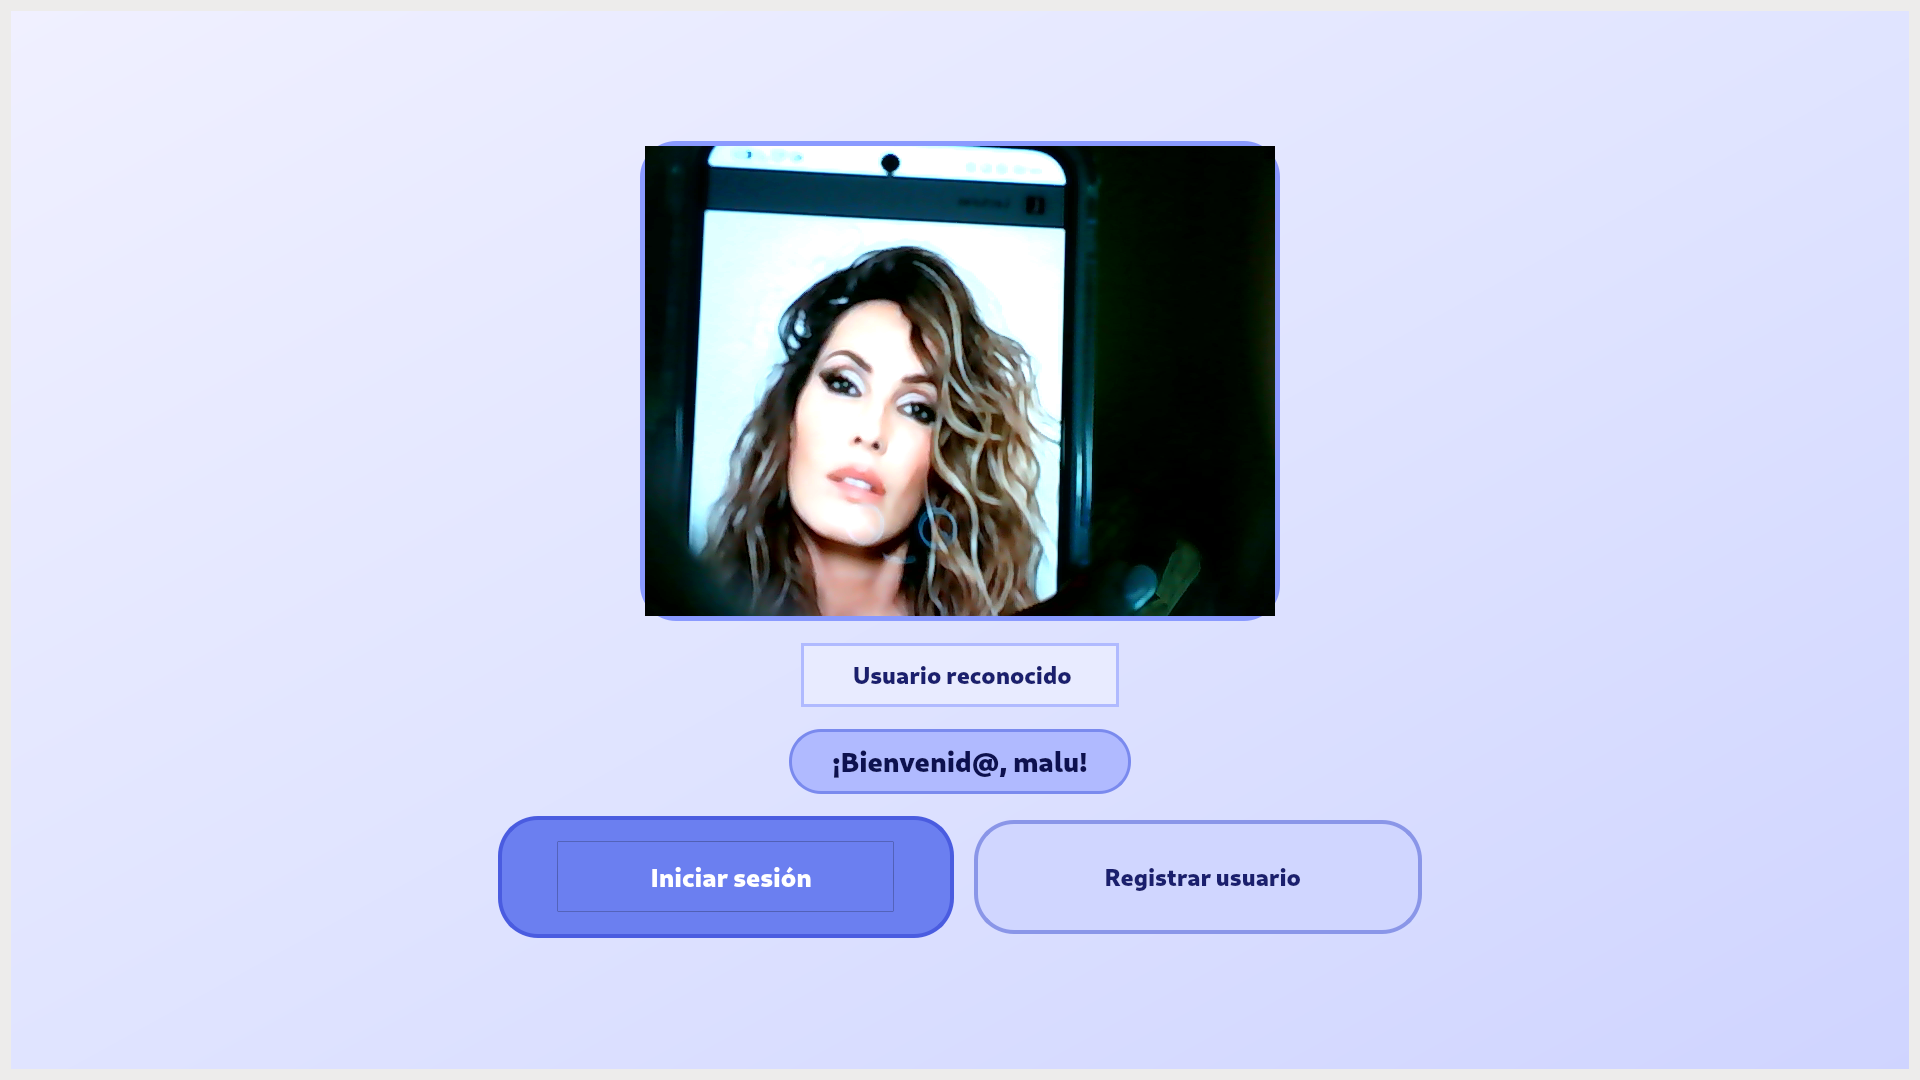
\includegraphics[width=15cm]{figs/logmal}
  \end{center}
  \caption{Pantalla de autenticación}
  \label{fig:logmal}
\end{figure}\

\begin{figure} [h!]
  \begin{center}
    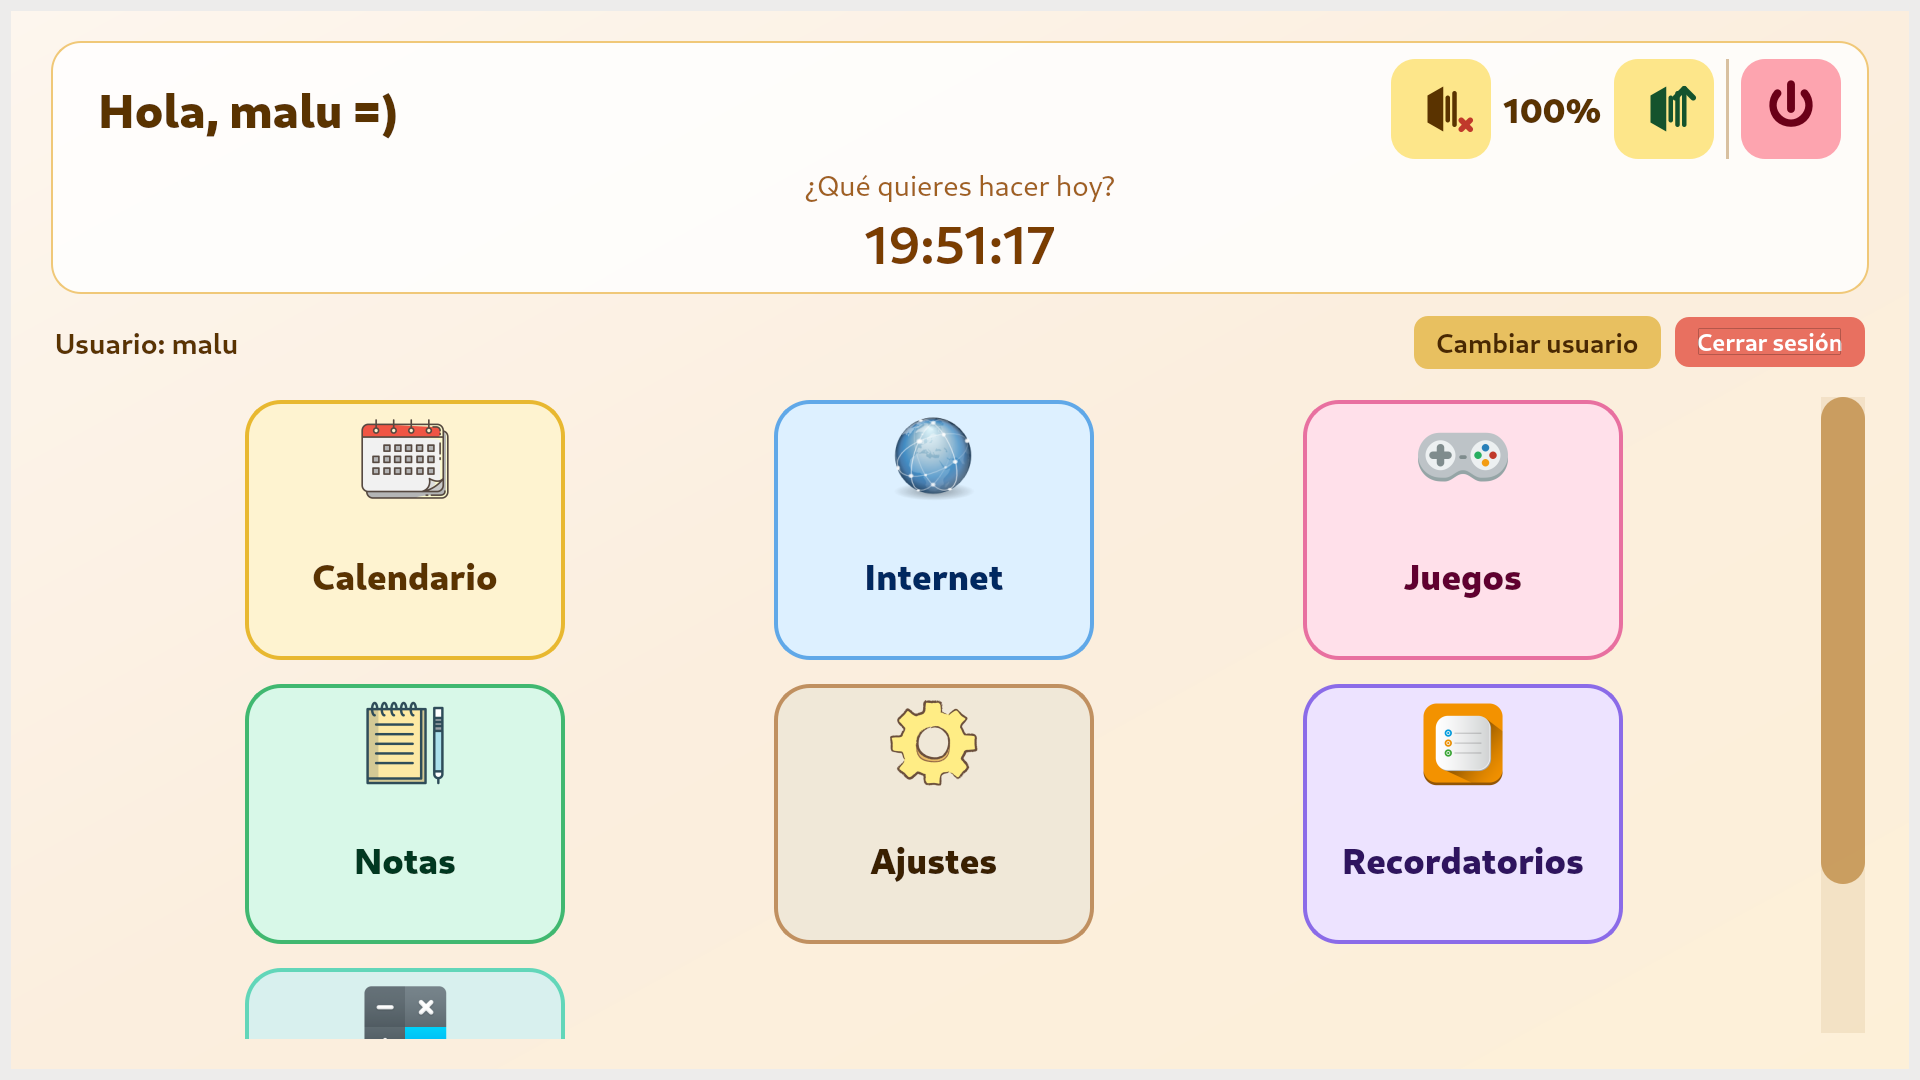
\includegraphics[width=15cm]{figs/logg}
  \end{center}
  \caption{Página principal del usuario identificado}
  \label{fig:logg}
\end{figure}\


\section{Modelo de lenguaje}
\label{sec:Modelo de lenguaje}

Una parte fundamental del robot es el sistema conversacional, ya que permite una interacción  más fluida y natural con el usuario. Por ello se han realizado pruebas centradas en la calidad de las respuestas y tiempo de respuesta, con el objetivo de evaluar su funcionamiento.

\vspace{0.2cm}

El modelo de lenguaje no se ejecuta de forma local, sino que se ejecuta en un servidor externo. Esto implica que cada interacción con el usuario sigue un flujo que incluye la captura de audio, el envío de peticiones al servidor, la generación de la respuesta y su transmisión al robot, donde es procesada y reproducida mediante síntesis de voz. Este proceso introduce latencia en el tiempo de respuesta del sistema del sistema.

\vspace{0.2cm}

Con el objetivo de evaluar el rendimiento, se realizaron pruebas comparando distintos modelos de lenguaje bajo las mismas condiciones de uso. Durante estas pruebas se registraron las respuestas obtenidas por cada modelo, así como la latencia, entendida como el tiempo transcurrido desde el envío de la petición hasta la recepción de la respuesta.

Los resultados obtenidos mostraron una gran diferencia entre modelos. En general, \textit{LLaMA 3} presentó un menor tiempo de respuesta y un comportamiento más estable, mientras que modelos como \textit{Gemini} presentaron mayor variabilidad en la latencia.


En el Cuadro~\ref{tab:llm_latency} se muestran los resultados obtenidos durante la evaluación en cuanto a la latencia.

\begin{table}[H]
\begin{center}
\begin{tabular}{|c|c|}
\hline
\textbf{Modelo} & \textbf{Latencia} \\
\hline
LLaMA 3 (Groq) & 0.7 - 2.5 s \\
\hline
GPT-4 (Azure) & 4 - 9 s \\
\hline
Gemini & 3 - 60 s (variable) \\
\hline
\end{tabular}
\caption{Comparativa de latencia entre modelos de lenguaje}
\label{tab:llm_latency}
\end{center}
\end{table}

Por otra parte, se evaluó la calidad de las respuestas generadas por el modelo con el objetivo de analizar su adecuación dentro del sistema conversacional. Para ello, se realizaron múltiples consultas en distintos ámbitos.

En general, \textit{LLaMA 3} generó respuestas coherentes y adecuadas al contexto de las preguntas planteadas.

A continuación se muestran algunos ejemplos de las respuestas obtenidas durante las pruebas:

\vspace{0.2cm}

\textbf{Ejemplo 1: Física (Relatividad)}

\begin{quote}
La teoría de la relatividad describe cómo el espacio y el tiempo no son absolutos, sino que dependen del observador. La velocidad de la luz es constante y el tiempo puede variar según la velocidad y la gravedad.
\end{quote}

\vspace{0.2cm}

\textbf{Ejemplo 2: Cine}

\begin{quote}
Te recomiendo algunas opciones clásicas y modernas que son consideradas muy escalofriantes: como \textit{El Exorcista (1973)}, \textit{La noche de los muertos vivientes (1968)}, \textit{El silencio de los corderos (1991)}, \textit{Get Out (2017)} o \textit{A Quiet Place (2018)}, películas muy intensas y aterradoras.
\end{quote}

\vspace{0.2cm}

\textbf{Ejemplo 3: Receta de cheesecake}
\begin{quote}
Ingredientes de cheesecake de fresa: galletas digestive molidas,  1/2 taza de azúcar,  1/4 taza de mantequilla derretida,  2 tazas de queso crema,  1/2 taza de azúcar, 2 huevos,  1 cucharadita de extracto de vainilla, 1 taza de puré de fresa,  1 taza de fresas frescas picadas.

\end{quote}

\vspace{0.2cm}

Estos resultados demuestran la efectividad del modelo de lenguaje dentro del sistema conversacional del robot, tanto en términos de calidad como de tiempos de respuestas.


\section{Sistema completo}
\label{sec:Sistema completo}

Finalmente, tras evaluar el funcionamiento de cada uno de los módulos de forma individual, se procedió a realizar pruebas del sistema completo.

\vspace{0.2cm}

\subsection{Arranque del sistema}

Durante el inicio del sistema, el robot intenta establecer conexión con el servidor. Cuando el servidor no se encuentra en ejecución, aparece  un error como el mostrado en el Código \ref{cod:inicio}.

\begin{code}[h]
\begin{lstlisting}[language=bash]

python -m app.main

pygame 2.1.2 (SDL 2.26.5, Python 3.11.2)
Hello from the pygame community. https://www.pygame.org/contribute.html
2026-06-26 13:21:07,911 - INFO - [MAIN] Iniciando sistema
[REMOTE LOG ERROR] HTTPConnectionPool(host='192.168.1.96', port=3000): Max retries exceeded with url: /client-log (Caused by ConnectTimeoutError(<urllib3.connection.HTTPConnection object at 0x7fa05367d0>, 'Connection to 192.168.1.96 timed out. (connect timeout=1)'))

\end{lstlisting}

\caption[Mensaje de error de conexión]{Mensaje de error de conexión}
\label{cod:inicio}
\end{code}


\subsection{Autenticación facial}

Tras el arranque, el sistema activa la cámara para realizar la autenticación facial del usuario. En la mayoría de las ejecuciones la cámara se inicializó correctamente y el sistema continuó sin incidentes. Sin embargo, en algunas ocasiones la cámara no se inicializó, provocando el bloqueo temporal del sistema. En estos casos fue suficiente con reiniciar la cámara y relanzar la aplicación.

Asimismo, se realizaron pruebas con distintos usuarios y con varias imágenes de una misma persona. El comportamiento fue satisfactorio en condiciones normales de iluminación (Figura \ref{fig:shaq}), exceptuando situaciones de baja intensidad lumínica (Figura \ref{fig:no_shaq}).

\begin{figure} [h!]
  \begin{center}
    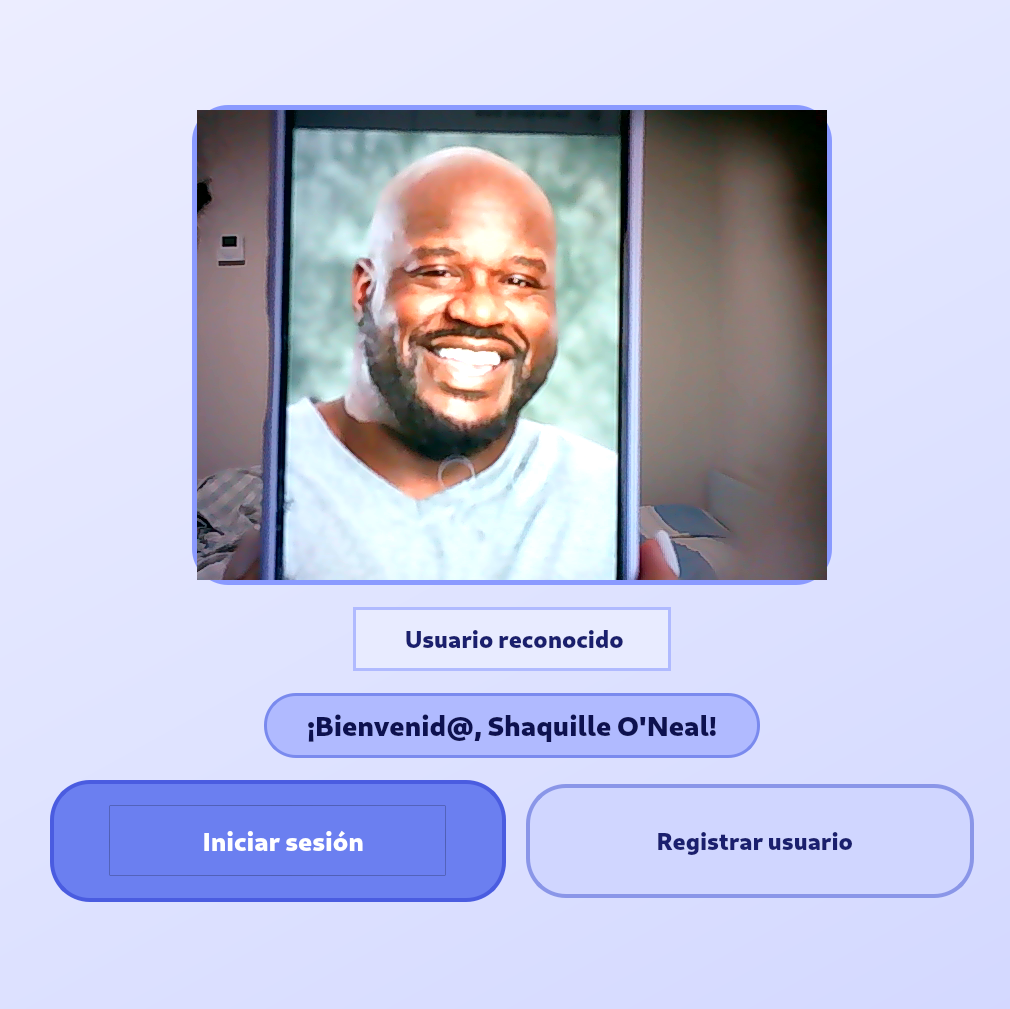
\includegraphics[width=8cm]{figs/shaq}
  \end{center}
  \caption{Condiciones del luz normales}
  \label{fig:shaq}
\end{figure}\

\begin{figure} [h!]
  \begin{center}
    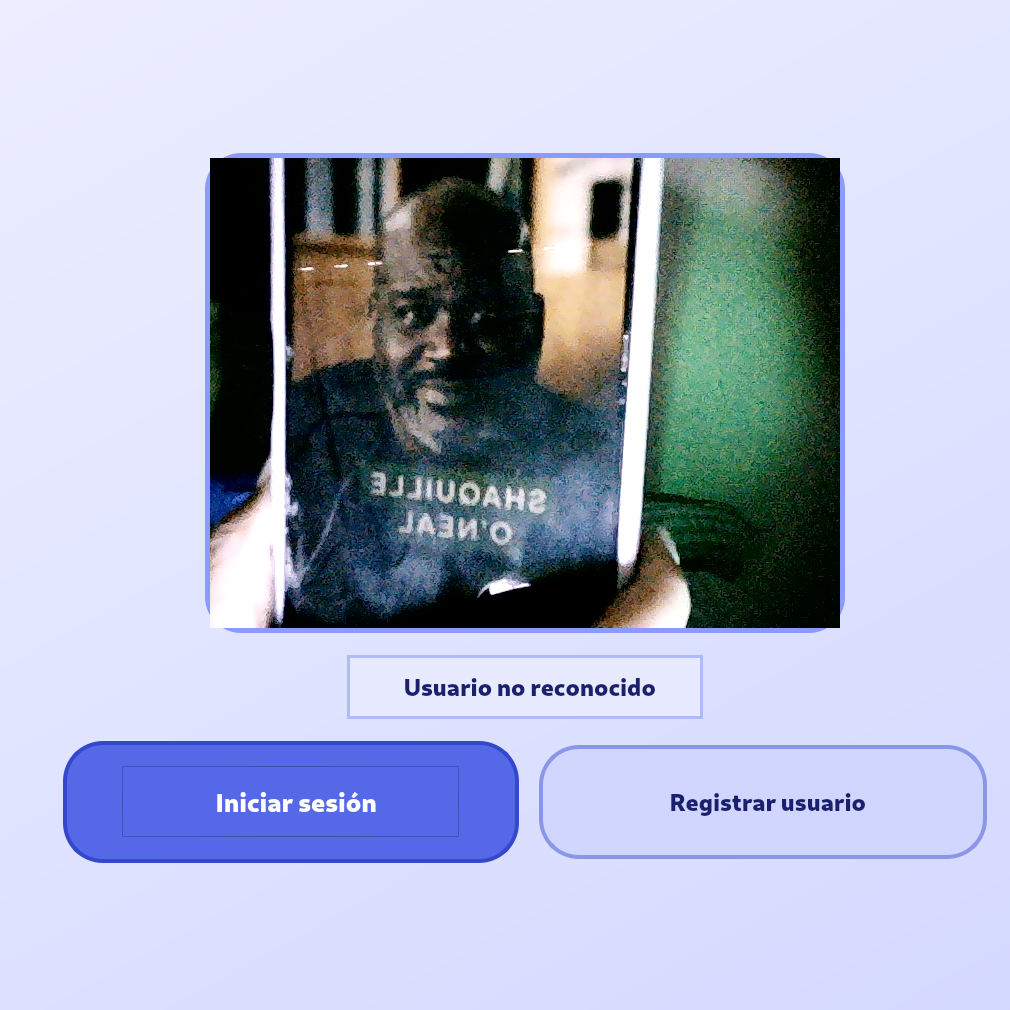
\includegraphics[width=8cm]{figs/no_shaq}
  \end{center}
  \caption{Baja luz}
  \label{fig:no_shaq}
\end{figure}\


\subsection{Activación mediante voz}

Una vez autenticado el usuario se habilita el acceso a las aplicaciones disponibles y el robot entra en modo de escucha, esperando la palabra de activación.

Durante el desarrollo se probaron diferentes palabras de activación debido a problemas de reconocimiento. Inicialmente se emplearon términos como ``Rojazz'' o ``Eliot'', pero fueron sustituidas por palabras más comunes y más reconocibles como ``asistente'', ``háblame'' u ``oye''.


\subsection{Sistema conversacional}

Una vez activado, el robot permite mantener conversaciones con el usuario.
Las primeras pruebas se centraron en consultas relacionadas con acontecimientos actuales, comprobando que el modelo de lenguaje era incapaz de responder debido a que no dispone de información posterior a su fecha de entrenamiento.

A continuación se presentan ejemplos que muestran algunas de las respuestas obtenidas ante consultas realizadas por el usuario:

\vspace{0.2cm}

\textbf{Ejemplo 1: Pregunta fútbol}

\begin{Verbatim}[breaklines=true]
USER:Elisa me puedes decir como quedó el partido españa uruguay

ROJAZZ: Lo siento, pero no tengo información en tiempo real sobre resultados de partidos. Mi conocimiento se basa en datos disponibles hasta mi última actualización, y no puedo proporcionarte el resultado del partido entre España y Uruguay. Sin embargo, puedo sugerirte algunas opciones para que puedas encontrar la información que buscas: Puedes intentar buscar en línea en sitios web de noticias deportivas o en la página oficial de la FIFA o de la selección de fútbol de España o Uruguay. También puedes intentar buscar en redes sociales como Twitter o Facebook, donde a menudo se comparten resultados y resúmenes de partidos. Si tienes una televisión o una tableta con acceso a internet, también puedes intentar buscar en canales de deportes o en aplicaciones de noticias deportivas para ver si tienen la información que buscas. ¿Quieres que te ayude a buscar en línea o te sugiera algún sitio web en particular donde puedas encontrar la información? Estoy aquí para ayudarte.
\end{Verbatim}


\textbf{Ejemplo 2: Pregunta fútbol}
\begin{Verbatim}[breaklines=true]
USER:Elisa cuento a mí como quedó alemania en el mundial hoy

ROJAZZ: Lo siento, pero no tengo información actualizada sobre el Mundial de fútbol o cualquier otro evento deportivo en tiempo real. Mi capacidad para proporcionar resultados o clasificaciones específicas de eventos deportivos es limitada, ya que no tengo acceso a información en tiempo real.Sin embargo, puedo sugerirte algunas opciones para que puedas enterarte de cómo quedó Alemania en el Mundial hoy: 1. Ver la televisión: Puedes intentar sintonizar un canal de noticias o deportes que esté cubriendo el Mundial. 2. Internet: Puedes buscar en internet en sitios web de noticias deportivas o en las páginas oficiales de la FIFA para obtener actualizaciones sobre el Mundial. 3. Aplicaciones móviles: Existen muchas aplicaciones móviles dedicadas a deportes que ofrecen resultados en tiempo real y noticias sobre eventos deportivos importantes.Espero que esta información te sea útil. ¿Hay algo más en lo que pueda ayudarte?
\end{Verbatim}

\vspace{0.2cm}

Con el objetivo de ampliar la funcionalidad, se incorporó un mecanismo de búsqueda de información en internet para determinadas consultas como conceptos generales o relacionada con personas. Sin embargo, consultas específicas como resultados deportivos, lo que requería el uso de técnicas de \textit{web scraping} o el uso de servicios de pago, por lo que se decidió no incorporar esta funcionalidad.

\vspace{0.2cm}

\textbf{Ejemplo 3: Consulta a internet}

\begin{Verbatim}[breaklines=true]
USER:Elisa quién es Napoleon

ROJAZZ: Napoleón Bonaparte (nacido Napoleone Buonaparte; Ajaccio, 15 de agosto de 1769-Santa Elena, 5 de mayo de 1821), más tarde conocido por su nombre regnal Napoleón I, fue un militar y político francés nacido en Córcega que saltó a la fama durante la Revolución francesa y dirigió exitosas campañas durante las guerras revolucionarias. Fue el líder de facto de la República francesa como primer cónsul desde 1799 hasta 1804, y después emperador de los franceses desde 1804 hasta 1814 y, de nuevo, en 1815. El legado político y cultural de Napoleón perdura, en tanto líder tan célebre como controvertido. Inició muchas reformas liberales que han perdurado en la sociedad, y se le considera uno de los más grandes comandantes militares de la historia. Sus campañas se estudian en las academias militares del mundo. Entre tres y seis millones de civiles y soldados murieron en lo que se conoció como las guerras napoleónicas. Espero que esta información te sea útil. ¿Hay algo más en lo que pueda ayudarte?
\end{Verbatim}


\subsection{Gestión de recordatorios y eventos}

Otra de las funcionalidades evaluadas fue el uso de la escucha activa para gestionar recordatorios y eventos por voz. Se realizaron pruebas tanto de creación como de consulta de recordatorios y eventos.

En la mayoría de los casos se interpretó correctamente las órdenes del usuario, aunque ocasionalmente se malinterpretaron las órdenes dando lugar a un resultado diferente al esperado.

Los siguientes ejemplos muestran algunos de los casos:

\vspace{0.2cm}

\textbf{Ejemplo 4: Consultar recordatorio}

\begin{Verbatim}[breaklines=true]
USER:Elisa tengo un recordatorio pendiente

ROJAZZ: Añadiendo a recordatorios
[REMINDER] 'un pendiente' → 20:47 28/06
\end{Verbatim}

\vspace{0.2cm}

\textbf{Ejemplo 5: Consultar recordatorio}

\begin{Verbatim}[breaklines=true]
USER:Elisa que alarmas tengo

ROJAZZ: Tienes 3 recordatorios pendientes: inyección a las 18:00, inyección tap a las 07:00, mi recordatorios a las 20:48.
\end{Verbatim}

\vspace{0.2cm}

\textbf{Ejemplo 6: Consultar recordatorio}

\begin{Verbatim}[breaklines=true]

USER:Elisa tengo recordatorios pendientes

ROJAZZ: Tienes 3 recordatorios pendientes: inyección a las 18:00, inyección tap a las 07:00, mi recordatorios a las 20:48.
\end{Verbatim}

\vspace{0.2cm}

\textbf{Ejemplo 7: Añadir evento}

\begin{Verbatim}[breaklines=true]
USER:Elisa recuérdame a las cinco pastillas

ROJAZZ: Recordatorio 'pastillas' añadido para las 05:00 del 29/06.
\end{Verbatim}

\vspace{0.2cm}

\textbf{Ejemplo 8: Añadir evento}

\begin{Verbatim}[breaklines=true]
USER:Elisa avísame a las cuatro de coche

ROJAZZ: Recordatorio 'coche' añadido para las 04:00 del 29/06.
\end{Verbatim}

\vspace{0.2cm}

\textbf{Ejemplo 9: Consultar eventos}

\begin{Verbatim}[breaklines=true]
USER:Elisa que tengo pendiente

(ROJAZZ) No tienes eventos el 28/06/2026.
\end{Verbatim}


\subsection{Evaluación global}

En conjunto, las pruebas realizadas permitieron validar el correcto funcionamiento del sistema integrado. El robot fue capaz de realizar el flujo completo, incluyendo el arranque de la aplicación, la autenticación facial, la activación del sistema conversacional, la gestión de eventos y recordatorios y el uso de las aplicaciones.


